\renewcommand\chapterillustration{abertura-afim}
\renewcommand\chapterwhat{Função exponencial, expoentes racionais e irracionais, crescimento e decaimento exponenciais, juros compostor, progressão geométrica.}
\renewcommand\chapterbecause{Dizemos que estamos diante de um crescimento exponencial sempre que o aumento percentual de determinada quantidade por unidade de tempo é constante. Este é o caso das medições econômicas, financeiras e poíticas de crescimento - de vendas, lucros, preços de ações, produto interno bruto, inflação, taxas de juros. Assim, compreender bem o crescimento exopnencial é crucial para compreender o mundo. As funções exponenciais são usadas para analisar e compreender problemas de diferentes áreas do conhecimento. Elas modelam o comportamento de epidemias e populações de um modo geral, são úteis na determinação da idade de fósseis e artefatos antigos, são aplicadas na ciência forense - uma área de estudo que se ocupa da análise científica das evidências de um crime - assim como em diversas outras aplicações.}
\chapter{Função Exponencial}



\mbox{}\thispagestyle{empty}\clearpage

\thispagestyle{empty}

\begin{center}
Projeto: LIVRO ABERTO DE MATEMÁTICA

\noindent \begin{tabular}{lcccr}

\includegraphics[scale=.15]{impa}& \quad\quad& 
\includegraphics[width=3cm]{logo} & \quad\quad& 
\includegraphics[scale=.24]{obmep} 
\end{tabular}
\end{center}

\vspace*{.3cm}

Cadastre-se como colaborador no site do projeto: \url{umlivroaberto.org}

Versão digital do capítulo:

\url{https://www.umlivroaberto.org/BookCloud/Volume_1/master/view/AF107.html}


\begin{tabular}{p{.15\textwidth}p{.7\textwidth}}
Título: & Função Exponencial\\
\\
Ano/ Versão: & 2020 / versão 1.0 de 24 de março de 2020\\
\\
Editora & Instituto Nacional de Matem\'atica Pura e Aplicada (IMPA-OS)\\
\\
Realização:& Olimp\'iada Brasileira de Matem\'atica das Escolas P\'ublicas (OBMEP)\\
\\
Produção:& Associação Livro Aberto\\
\\
Coordenação:& Fabio Simas, \\
            & Augusto Teixeira (livroaberto@impa.br)\\
\\
  Autores: & Gladson Antunes (UNIRIO),\\
        & Michel Cambrainha (UNIRIO),\\
             & Bruno Vianna (Colégio Pedro II).\\
\\
Revisão: &  Cydara Ripoll  \\
         &  Letícia Rangel \\
\\
Design: & Andreza Moreira (Tangentes Design) \\
\\
  Ilustrações: & Miller  Guglielmo \\ 
\\
Gráficos: & Beatriz Cabral e Tarso Caldas (Licenciandos da UNIRIO)\\
\\
  Capa: & Foto de Scott Webb, no Unplash \\
        & https://unsplash.com/photos/fMUIVein7Ng \\

\end{tabular}



\begin{figure}[b]
\begin{minipage}[l]{5cm}
\centering

{\large Licença:}

  
\includegraphics[width=3.5cm]{cc-by-sa1}
\end{minipage}\hfill
\begin{minipage}[c]{5cm}
\centering
{\large Desenvolvido por}


\includegraphics[width=2.5cm]{logo-associacao.jpg}
\end{minipage}
\begin{minipage}[r]{5cm}
\centering

{\large Patrocínio:}
  \vspace{1em}
  
\includegraphics[width=3.5cm]{itau}
\end{minipage}
\end{figure}

\mainmatter

\explore{Crescimento e Decaimento exponenciais}

A pandemia de COVID-19, uma doença respiratória aguda provocada pelo coronavírus SARS-CoV-2, chamou a atenção do mundo todo em 2020 para o que chamamos de crescimento exponencial. Vimos diversos especialistas em diferentes meios de comuncação comentando sobre o crescimento exponencial da epidemia. Mas afinal, o que caracteriza este tipo de crescimento?

% \begin{multicols}{2}
% \begin{figure}[H]
% \centering

% 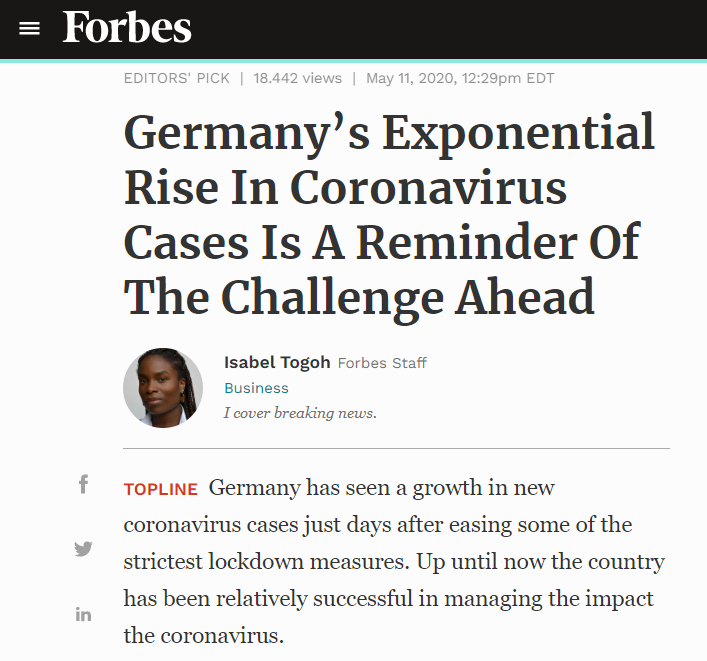
\includegraphics[width=150bp]{Figuras/exponencial1.png}
% \end{figure}


% \begin{figure}[H]
% \centering

% 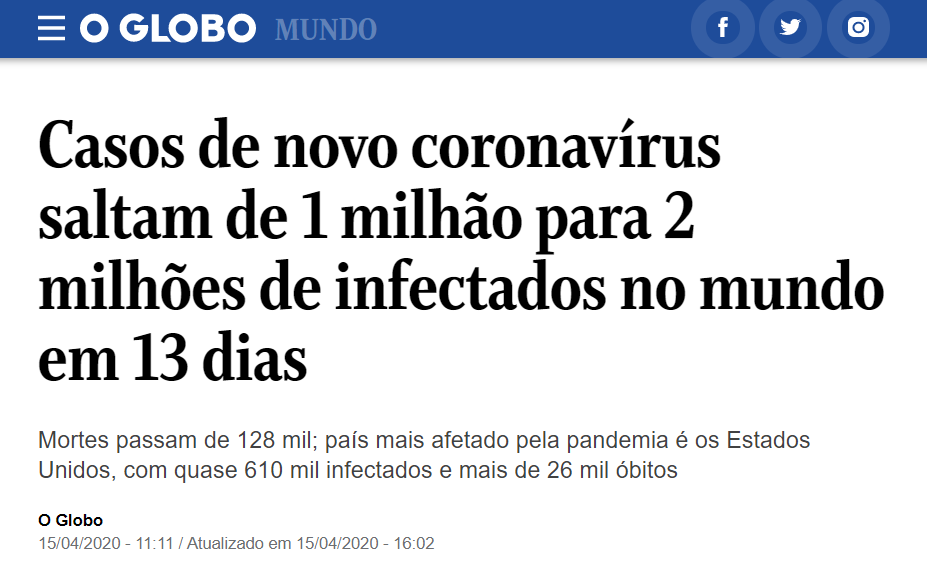
\includegraphics[width=2300bp]{Figuras/exponencial2.png}
% \end{figure}

% \end{multicols}



\begin{minipage}{0.4\textwidth}
\begin{figure}[H]
\centering

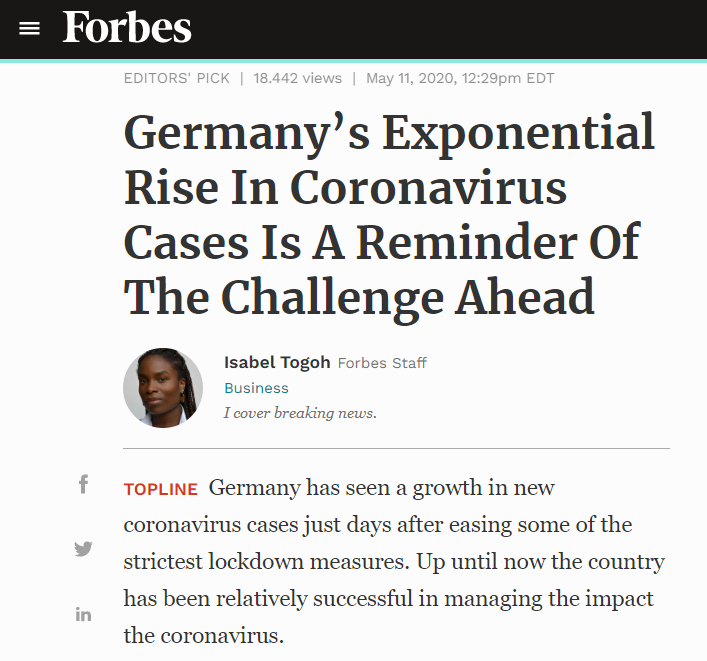
\includegraphics[width=150bp]{Figuras/exponencial1.png}
\end{figure}
\end{minipage}
\begin{minipage}{0.6\textwidth}
\begin{figure}[H]
\centering

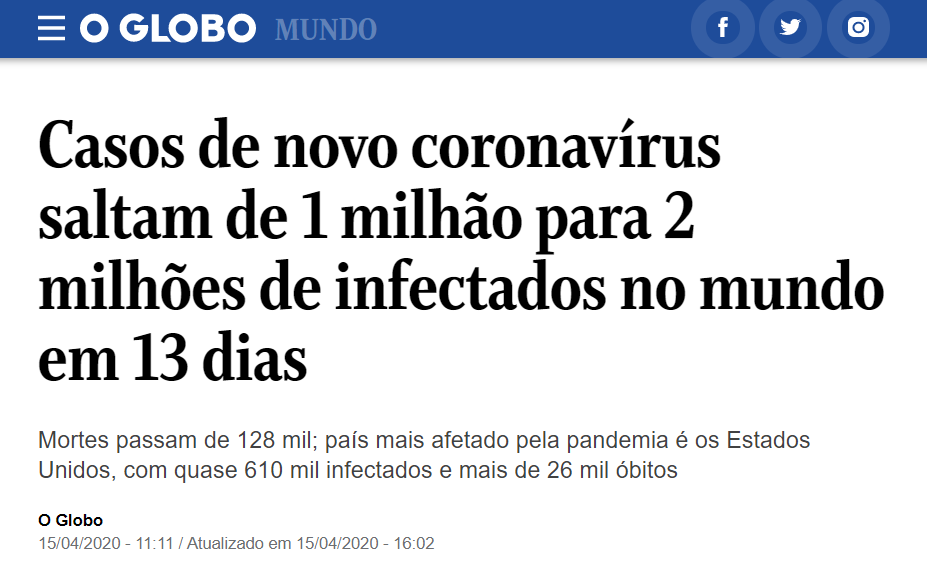
\includegraphics[width=230bp]{Figuras/exponencial2.png}
\end{figure}

\end{minipage}


Sabemos que funções matemáticas podem ser usadas para fazermos previsões de um determinado fenômeno. A função exponencial fornece um modelo matemático simples para calcular a propagação de uma doença. Para além disso, o gráfico de uma função exponencial permite o estudo de situações que se caracterizam por uma curva de crescimento ou decrescimento acentuado. Neste capítulo você irá aprender a identificar, elaborar e resolver problemas que envolvem funções exponenciais. Além da modelagem de epidemias, serão apresentadas situações que envolvem decaimento radioativo, meia-vida de medicamentos, pressão atmosférica, divisão celular, dentre outras aplicações interessantes.

\begin{task}{epidemias}

\begin{figure}[H]
\centering

\includegraphics[width=300bp]{exponencial3}

\end{figure}

Vamos simular três situações de epidemia. O professor irá distribuir envelopes contendo um número para cada estudante que deverá mantê-lo em segredo. Os primeiros infectados serão escolhidos ao acaso pelo professor. Cada vez que alguém for infectado pela doença, doloca-se de pé e permanece até o fim da dinâmica, que seguirá da seguinte maneira:

\textbf{Epidemia 1}
\begin{itemize}
\item \textbf{Rodada 0}: O professor escolhe \textbf{dois} números para serem os primeiros infectados, diz seus números e apaga-os da lista que está escrita na lousa. Os infectados ficam de pé. O pesquisador anota o número de infectados.
\item\textbf{Rodada 1}: Cada um dos infectados escolhe \textbf{um} número que não tenha sido sorteado para "infectar"; os números são apagados na lousa e somente depois de todos terem escolhido suas vítimas, os novos infectados se colocam de pé. O pesquisador anota o número total de infectados.
\item\textbf{Rodada 2}: Semelhante à rodada 1.
\item As rodadas seguem até que todos tenham sido infectados.
\end{itemize}

\textbf{Epidemia 2}
\begin{itemize}
\item A mesma dinâmica anterior, porém começando com \textbf{três} infectados na rodada 0.
\end{itemize}


\textbf{Epidemia 3}
\begin{itemize}
\item Apenas \textbf{um infectado} na rodada 0 e cada infectado agora escolhe \textbf{dois} números para infectar a cada rodada.
\end{itemize}

Responda as seguintes perguntas:

\begin{enumerate}
\item Anote os dados das três epidemias em tabelas e faça previsões para quatro rodadas além das que efetivamente ocorreram na sua turma.
\item Represente os dados graficamente.
\item Que critérios você usou no item a) para fazer suas previsões? Qual a relação deles com os dados específicos de cada uma das epidemias.
\item Quanto tempo aproximadamente demoraria para cada epidemia infectar todos os estudantes da sua escola? Primeiro faça um "chute" e somente depois faça as contas.
\item Responda a mesma pergunta anterior considerando a sua cidade, seu estado e todo o país.
\end{enumerate}
\end{task}


\begin{task}{Contando quadrados}

Em uma caixa há 240 quadradinhos de papel cartão dupla face, verde de um lado e marrom do outro. Eles são lançados sobre a mesa e os quadrados com lado marrom para cima são retirados, restando apenas 126 quadradinhos (verdes). Um novo lançamento é feito depois de retirados os marrons, sobram 68 verdes. Os lançamentos seguintes apresentam as seguintes quantidades de quadradinhos verdes:

\begin{table}[H]
\centering
\begin{tabu} to \textwidth{|c|c|}
\hline
\thead
Lançamento & \# Verdes \\
\hline
0 & 240 \\
\hline
1 & 126 \\
\hline
2 & 68 \\
\hline
3 & 34 \\
\hline
4 & 13 \\
\hline
5 & 5 \\
\hline
6 & 2 \\
\hline
7 & 0 \\
\hline
\end{tabu}
\end{table}

\begin{enumerate}
\item Represente em um sistema de coordenadas os dados da tabela acima.
\item Observando os dados da tabela é possível conjecturar que eles obedecem a algum padrão?
\item Acrescente uma terceira coluna à tabela contendo os quocientes entre as quantidades de um lancamento pela quantidade do lançamento anterior.

\begin{table}[H]
\centering
\setlength\tabulinesep{2.5pt}
\renewcommand{\arraystretch}{1.75}
\begin{tabu} to \textwidth{|c|c|c|}
\hline
\thead
Lançamento & \# Verdes & Quocientes\\
\hline
0 & 240 & ---\\
\hline
1 & 126 & $\displaystyle\frac{126}{240}\approx0,525$\\
\hline
2 & 68 & \\
\hline
3 & 34 & \\
\hline
4 & 13 & \\
\hline
5 & 5 & \\
\hline
6 & 2 & \\
\hline
7 & 0 & \\
\hline
\end{tabu}
\end{table}

\item Considerando outros resultados possíveis para o mesmo experimento, o que podemos esperar dos valores na terceira coluna da tabela? Que tipo de propriedades matemáticas esses números \textbf{sempre} terão? Que tipo de propriedade eles \textbf{provavelmente} terão?
\item Um experimento como este descrito no item a) pode ser simulado computacionalmente. Ao executar esta simulação quatro vezes, os seguintes resultados foram obtidos.

240, 113, 55, 28, 13, 7, 3, 0

240, 124, 66, 27, 16, 7, 3, 2, 2, 2, 0

240, 105, 57, 19, 9, 5, 1, 0

240, 124,  62, 29, 11, 5, 2, 1, 1, 0

Verifique se suas conjecturas se aplicam aos dados acima.

\item Deduza uma expressão matemática que forneça, aproximadamente, a quantidade de quadradinhos verdes em função da ordem de lançamento.

\end{enumerate}


\end{task}

\begin{task}{Populações}

Um grupo de biólogos está estudando uma espécie animal cuja população vem diminuindo ao longo dos anos. Depois de reunirem os dados percebem que a cada ano a quantidade de indivíduos reduz aproximadadamente $1/3$ da quantidade do ano anterior.

\begin{enumerate}
\item Escreva uma expressão matemática que relaciona o número de indivíduos dessa população ao longo dos anos, sabendo que no início das medições os cientistas tenham encontrado 300 mil indivíduos.

\item Admitindo que esse padrão se repita ao longo dos anos, em quanto tempo a população entrará em extinção?

\item Como consequência, a população da espécie que é a principal presa da espécie estudada apresentou um crescimento que duplicava a cada seis meses. Escreva uma expressão matemática que represente a variação anual do número de indivíduos dessa população de presas, que no início das medições contava com $5\times 10^5$ indivíduos.
\end{enumerate}

\end{task}

\arrange{Crescimento e Decaimento exponenciais}

Nos capítulos anteriores conhecemos diversas situações e fenômenos descritos por funções lineares ou polinomiais. No entando, há muitas outras situações em que estas funções não se mostram as mais adequadas para a modelagem. Mas que situações seriam estas? Pelo que foi visto nas atividades anteriores, são aquelas para as quais observamos um rápido crescimento ou um rápido decrescimento. O mais interessante é que situações e fenômenos com estas características são abundantes nas mais diferentes áreas do conhecimento.

Vejamos um novo exemplo: o crescimento das plantas é um processo ecológico fundamental. A análise do crescimento das plandas (que inclui a determinação de parâmetros que descrevem suas taxas de crescimento) se constitui uma importante área de pesquisa em ecologia. Melhorias recentes na modelagem deste processo permitiram uma compreensão mais profunda e previsões mais precisas para uma ampla gama de questões, incluindo competição entre plantas, interações planta-herbívoro e funcionamento de ecossistemas.Para muitas especies de plantas, durante algum período de tempo,. no início de seu desenvolvimento, observa-se esse tal crescimento rápido, que chamamos de exponencial.

\begin{figure}[H]
\centering
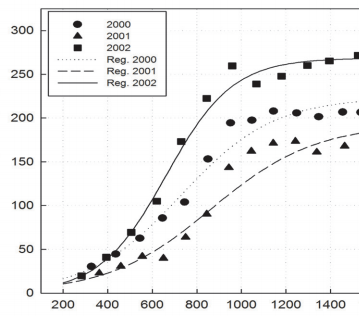
\includegraphics[width=200bp]{exponencial4}

\end{figure}

\begin{reflection}

O crescimento exponencial pressupõe recursos ilimitados e isso faz com que em muitos casos esse tipo de comportamento seja observado apenas em certos períodos de tempo. Isso pode ser visto, por exemplo, na forma como cresecem populações. Com ou pou ou sem nenhuma limitação de recurso populações podem apresentar um crescimento exponencial. No entanto, na prática sabemos que há uma série de limitações - espaço limitado, existência de predadores, escassez de alimentos, etc. - é o que os pesquisadores costumam chamar de \textit{Resistência Ambiental}. Portanto, após experimentar um período de crescimento exponencial, o que observamos é que a população tende a se estabilizar. Esse comportamento é chamado de crescimento logístico."

\begin{figure}[H]
\centering
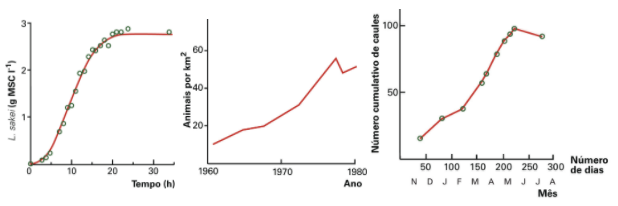
\includegraphics[width=400bp]{exponencial5}

\caption*{Exemplos reais de um aumento populacional como descrito acima. (a) a bactéria \textit{Lactobacillus sakei} crescendo em um meio de cultura. (b) A população de gnu, na região do Seringueti na Tanzânia. (c) População de juncácea anual, \textit{Juncus gerardi}.

Fonte: CEPA}
\end{figure}

\end{reflection}


Como, afinal identificamos o crescimento (ou decaimento) exponencial? Em todos os casos analisados nas atividades da seção anterior, observamos dois ingredientes fundamentais: um \textbf{valor inicial} para a variável dependete, decorre da primeira medição, e um valor constante positivo que servia como \textbf{fator de multiplicação} para se obter os valores seguintes.

\begin{figure}[H]
\centering
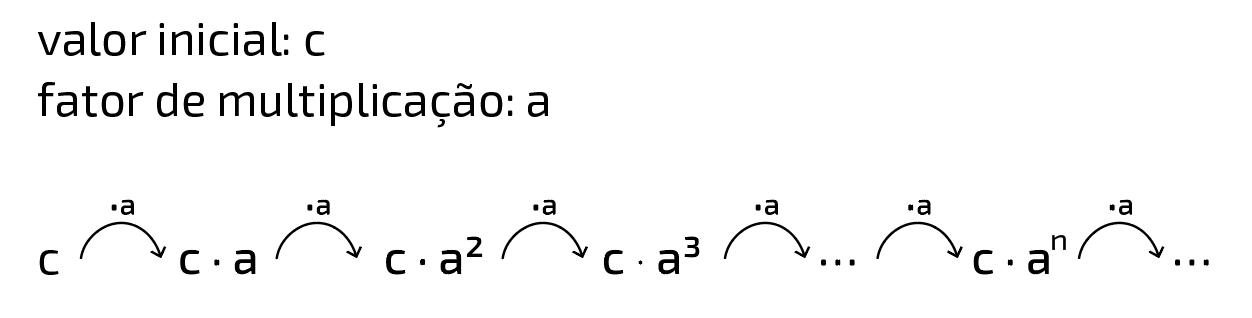
\includegraphics[width=350bp]{exponencial6}

\end{figure}


\begin{wrapfigure}{l}{.4\textwidth}

\centering

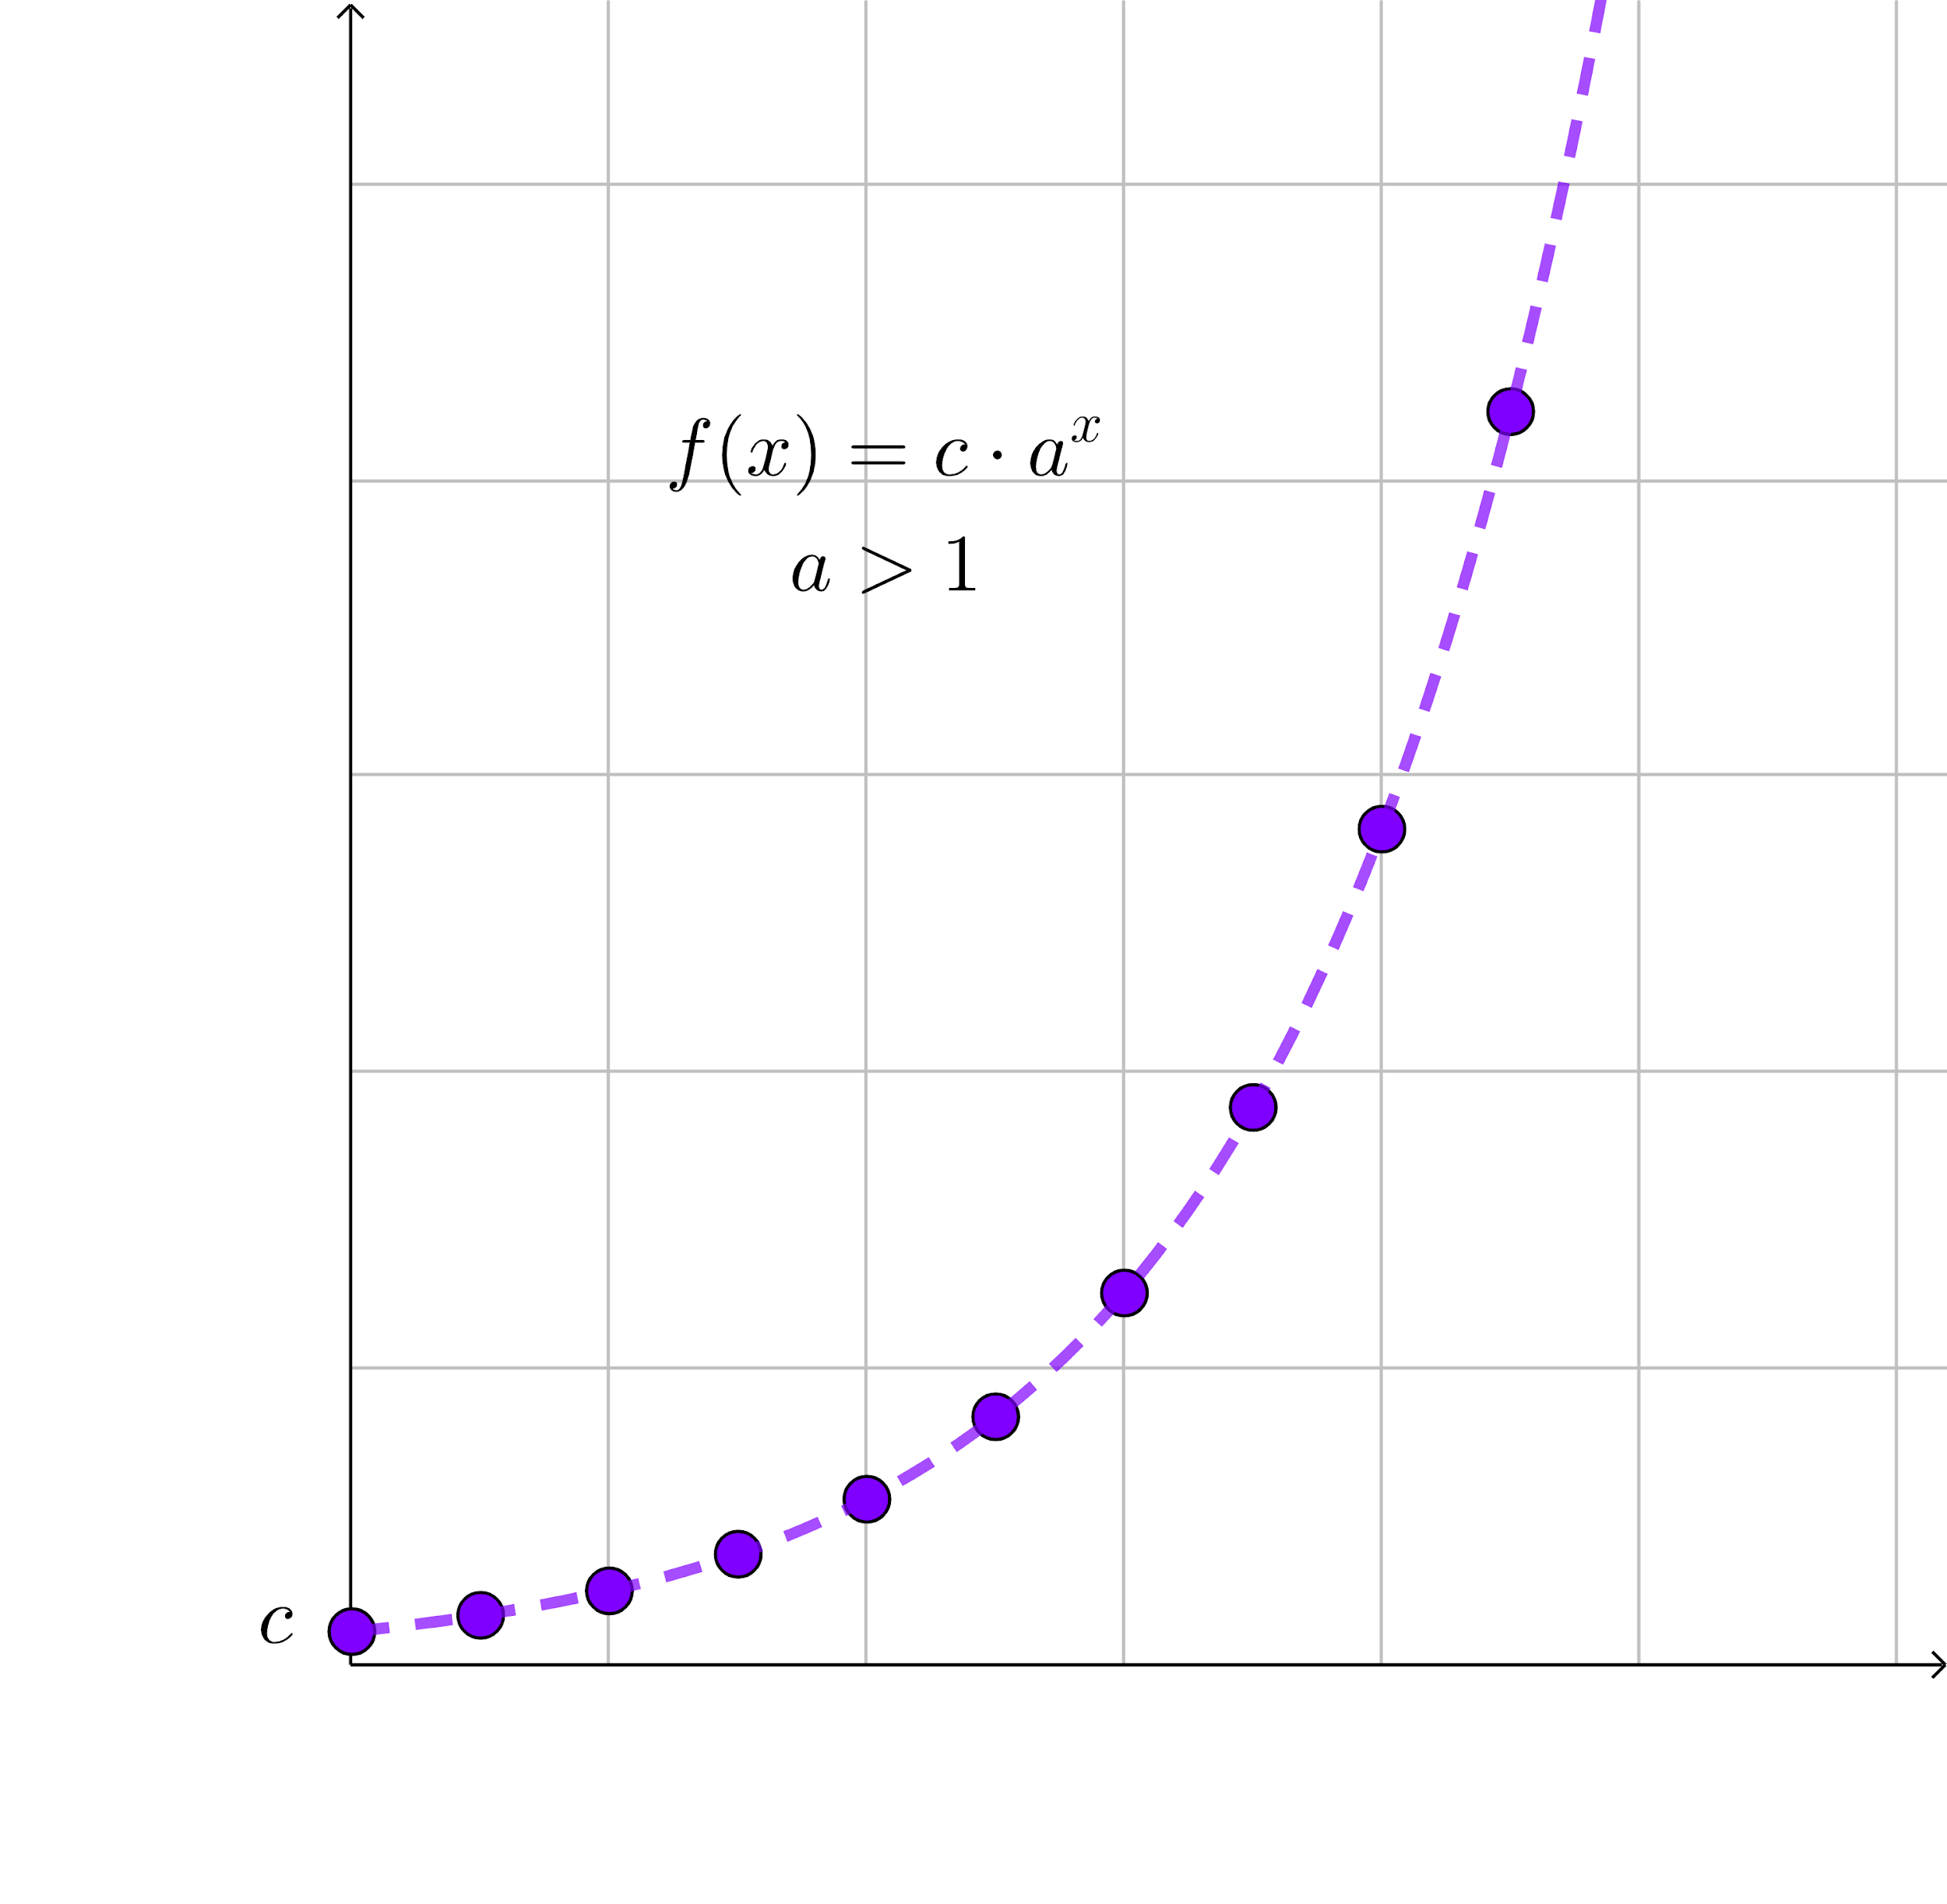
\includegraphics[width=.4\textwidth]{Figuras/exponencial7.png}

\end{wrapfigure}

Quando esse fenômeno ocorre estamos diante do crescimento ou decaimento exponencial, às vezes também chamado de progressão geométrica. Assim, a expressão

\begin{equation*}
f(x)=c\cdot a^x
\end{equation*}

é a que usamos para modelar situações em que há crescimento/decaimento exponencial.

Vamos, por ora, considerar que o valor inicial $c$ é igual a $1$ (se pensarmos em termos percentais, o valor inicial representa $100\%=1$, por exemplo). 


\clearpage
{
\begin{wrapfigure}{r}{.4\textwidth}

\centering
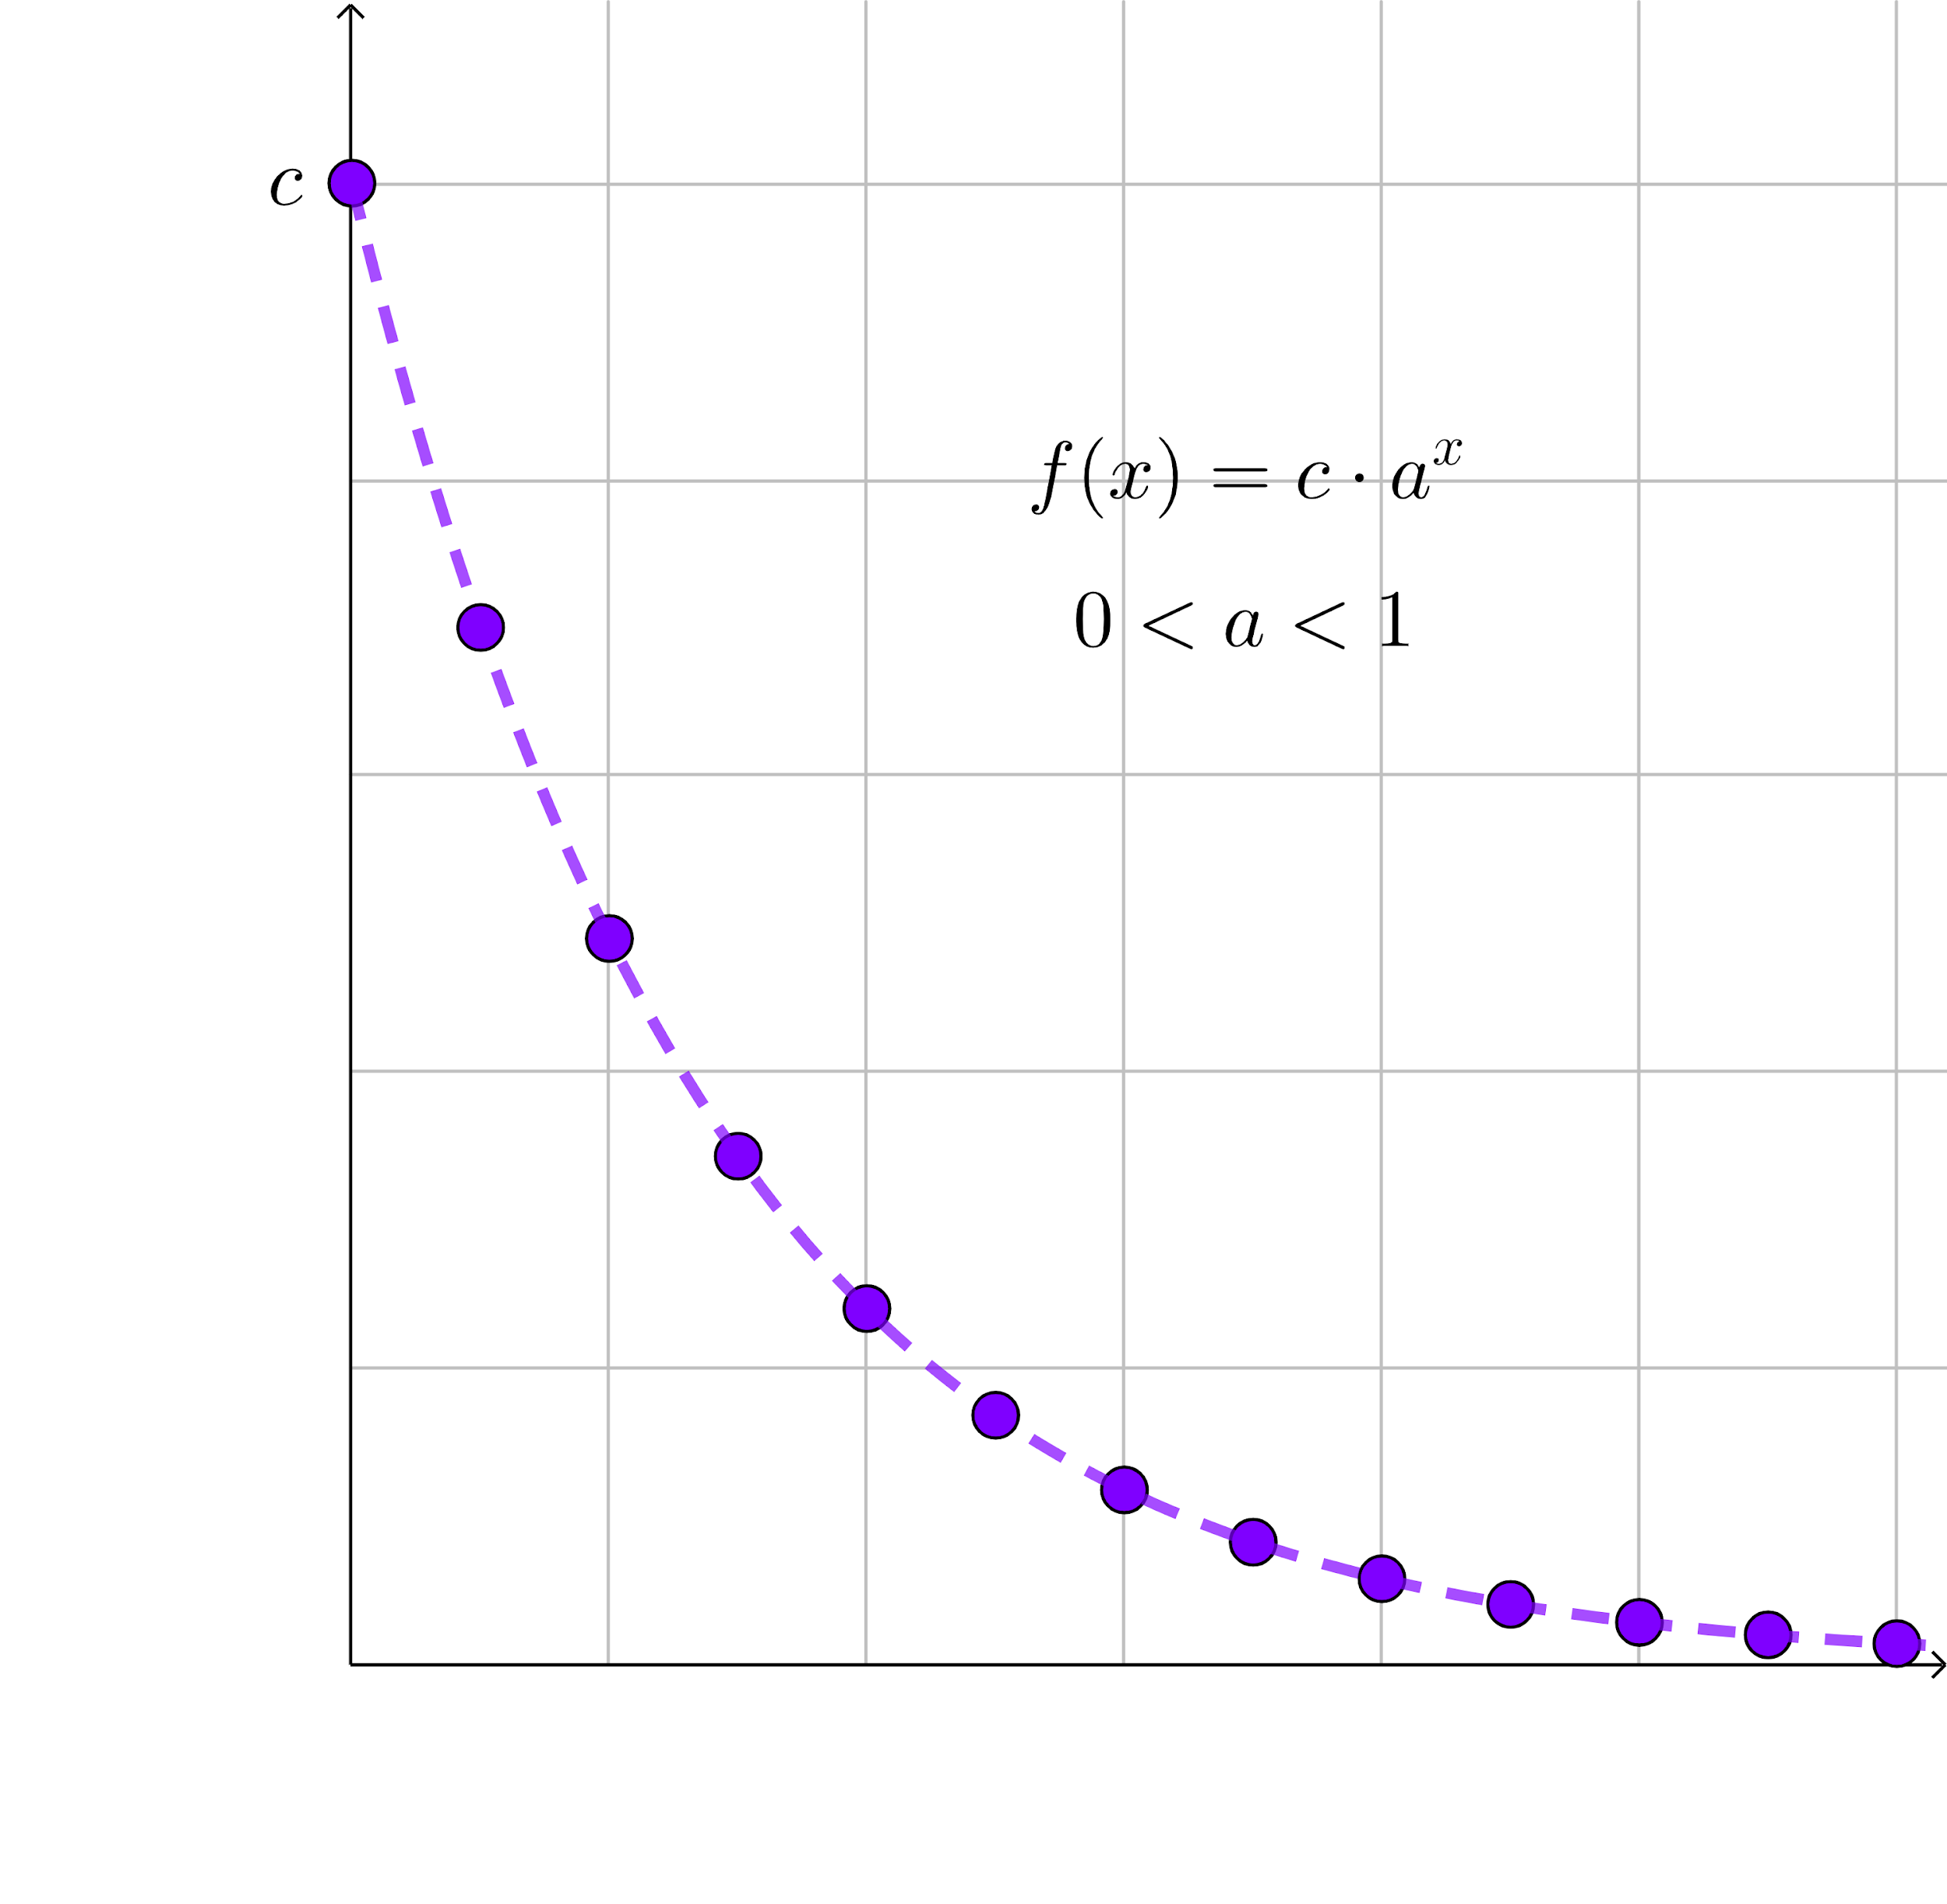
\includegraphics[width=.4\textwidth]{Figuras/exponencial8.png}

\end{wrapfigure}

Para que se observe de fato um crescimento, é necessário e suficiente que o fator multiplicativo seja um número maior que $1$.

\begin{equation*}
a > 1 \iff a^2>a \iff a^3>a^2 \iff ...
\end{equation*}

E de maneira análoga, veremos decaimento quando o fator é um número maior que zero e menor que 1.

\begin{equation*}
a<1 \iff a^2<a \iff a^3<a^2 \iff ...
\end{equation*}

\url{https://www.desmos.com/calculator/59ikonr8az}}

\begin{knowledge}

\begin{figure}[H]
\centering
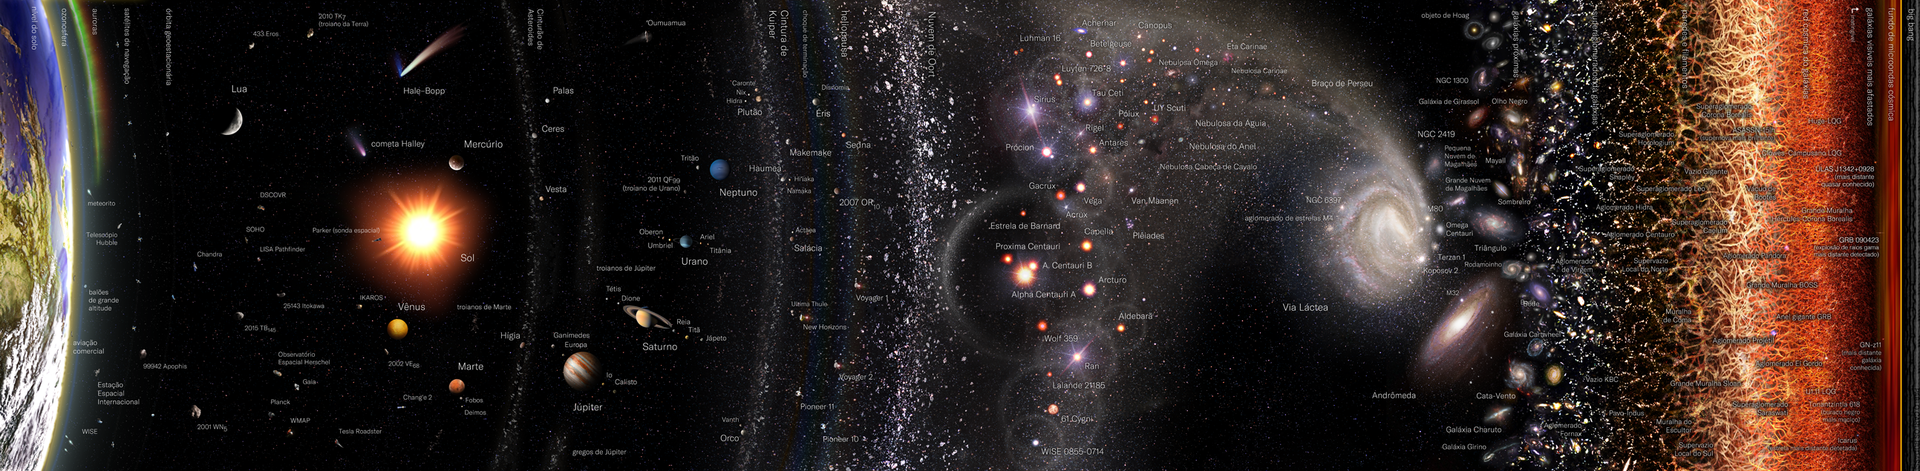
\includegraphics[width=400bp]{exponencial9}

\caption*{Por Pablo Carlos Budassi - Obra do próprio, CC BY-SA 4.0, \url{https://commons.wikimedia.org/w/index.php?curid=74584500}}
\end{figure}

O crescimento exponencial é tão rápido que com poucas multiplicações podemos alcançar valores cujas ordens de grandeza sãso maiores que a quantidade de átomos estimada para o universo observável (que é algo em torno de $10^80$).

\begin{wrapfigure}{l}{.4\textwidth}

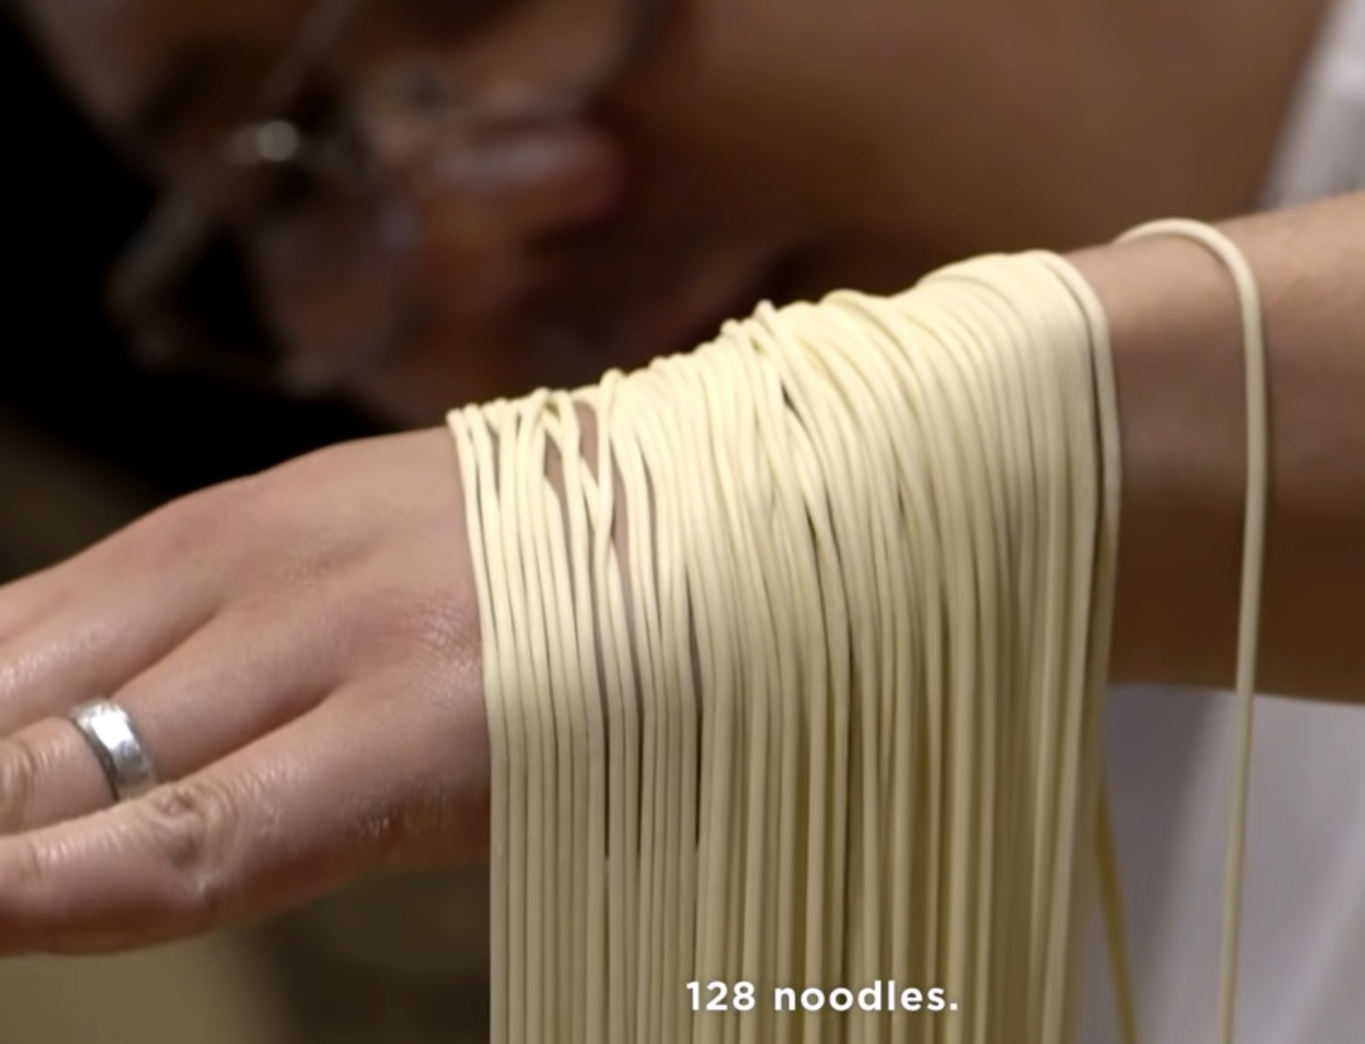
\includegraphics[width=.4\textwidth]{Figuras/exponencial10.png}

\end{wrapfigure}

Nesse vídeo, um chef de cozinha chinês faz 128 em apenas 10 segundos! \url{https://youtu.be/S2AnYEheaFM?t=120}.

Vejamos um outro exemplo para entender o quão rápido é o crescimento exponencial. Pegue com uma folha de papel sulfite (ou do seu caderno), cuja espessura é algo em torno de $0,075$ milímetros. Se dobramos essa folha ao meio, temos o dobro da espessura inicial, $0,15$ mm. Dobrando novamente, $0,30$ mm e assim sucessivamente.

Nenhum ser humano, usando somente as mãos consegue dobrar uma folha dessas mais que seis vezes, pode tentar! Uma folha dobrada 7 vezes tem a espessura de um caderno de 128 páginas... E mais, se fosse possível dobrar a folha 23 vezes, a espessura seria maior que a distância da terra até a Lua.

E aí? Com quantas dobras a espessura alcançaria a ordem de grandeza do número de átomos do universo conhecido?
\end{knowledge}

A área de Computação parece desafiar o fato de que não é possível manter um cresecimento exponencial por um longo período de tempo devido à escassez de recursos. Talvez o processo exponencial mais longo de que se tem notícia na natureza se refere ao crescimento do poder computacional disponível por 1 US\$. Este parâmetro vem seguindo uma exponencial crescente constante de tempo de aproximandamente 18 meses e que vem sendo observada desde o lançamento dos primeiro computadores comerciais em meados da década de 1950. Ou seja, desde esta época, até o início dos anos 2000, houve uma duplicação do poder computacional disponível por 1 US\$ vezes seguidas, ou seja, uma variação de 134 milhões de vezes em 40 anos. Estes números são aproximados, pois não conhecemos um estudo preciso nesta direção, no termos descritos.

Uma outra lei similar é conhecida como lei de Moore. Gordon Moore foi um dos fundadores da Intel, uma das maiores fabricantes mundiais de circuitos integrados. Ele enunciou a sua lei de 1965, numa época em que um microchip podia integrar algo como 4 transistores: \textbf{"o desempenho de microchips produzidos em massa vai dobrar a cada 18 meses"}. Aqui o limitante de preço é substituído pela condição de produção em massa, o que dá um efeito similar, já que só é possível produzir em massa componentes suficientemente baratos para poderem ser absorvidos pelo mercado.

\practice{Crescimento e Decaimento exponenciais}


\begin{task}{A fazenda de árvores}

Uma fazendo de árvores começou a colher um lote que havia sido plantada anos atrás. A tabela abaixo mostra o número de árvores remanescentes para cada um dos 8 anos de colheita.

\begin{table}[H]
\centering
\setlength\tabulinesep{4pt}
\begin{tabu} to \textwidth{|m{.15\textwidth}|c|c|c|c|c|c|c|c|c|}
\hline
\centering\cellcolor{white}\textcolor{black}{\textbf{Ano}} & 0 & 1 & 2 & 3 & 4 & 5 & 6 & 7 & 8 \\
\hline
\centering\cellcolor{white}\textcolor{black}{\textbf{Árvores remanescentes}} & 10 000 & 9 502 & 9 026 & 8 674 & 8 145 & 7 737 & 7350 & 6982 & 6634 \\
\hline
\end{tabu}
\end{table}

\begin{enumerate}
\item Escreva uma expressão para função que relaciona as árvores remanescentes como tempo decorrido.
\item Analise os dados da tabela e fá uma previsão para os próximos anos mostrados na tabela a seguir:

\begin{table}[H]
\centering
\setlength\tabulinesep{4pt}
\begin{tabu} to \textwidth{|m{.15\textwidth}|*{8}{>{\centering}m{.07\textwidth}|}}
\hline
\centering\cellcolor{white}\textcolor{black}{\textbf{Ano}} & 10 & 15 & 20 & 25 & 30 & 35 & 40 \\
\hline
\centering\cellcolor{white}\textcolor{black}{\textbf{Árvores remanescentes}} &  & &  &  &  &  &  \\
\hline
\end{tabu}
\end{table}

\item Os donos da fazenda quere para a colheita quando sobrarem 15\% do número inicial de árvores do lote. Quando devem parar?

\end{enumerate}
\end{task}
\begin{task}{Cara ou coroa?}

Na teoria das probabilidades, ao analisar as chances de um determinado evento acontecer, é comum considerarmos todas as possibilidades para assim podermos quantificar a probabilidade. O conjunto formado por todas essas possibilidades é chamado de \textbf{espaço amostral}.

Você possui uma moeda, vai girá-la no ar e analisar qual vaçe ficou voltada para cima quando ela cair. O espaço amostral desse experimento contém dois elementos:\{cara (C), coroa (K)\}. Responda:

\begin{enumerate}
\item Qual o espaço amostral para o experimento de lançar a mesma moeda duas vezes?
\item E três vezes?
\item Explique a seguinte afirmação: 

"O tamanho do espaço amostral do lançamento de uma moeda várias vezes ao ar aumenta exponencialmente a relação a quantidade de lançamentos".
\end{enumerate}

\end{task}

\begin{task}{dobraduras}

Uma folha de papel de área $1$ é dobrada em três partes iguais, depois em mais três partes iguais, em terços novamente e assim sucessivamente.

\begin{figure}[H]
\centering
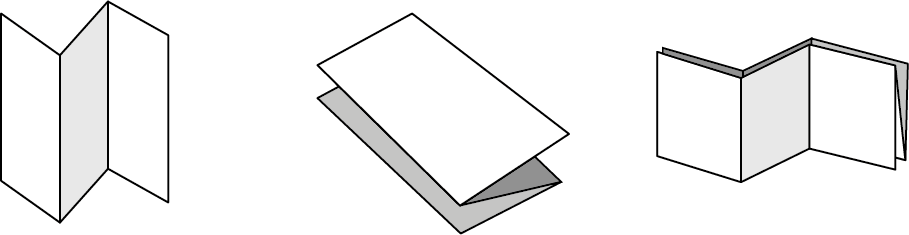
\includegraphics[width=300bp]{exponencial11}

\end{figure}

\begin{enumerate}
\item Na tabela a seguir, registre a área da menos região em cada etapa, e o número total de regiões.


\begin{table}[H]
\centering
\begin{tabu} to \textwidth{|c|c|c|}
\hline
\thead
Etapas & Área de cada região & Número de regiões \\
\hline
0 & 1 & 1 \\
\hline
1 & & \\
\hline
2 & & \\
\hline
3 & & \\
\hline
4 & & \\
\hline
5 & & \\
\hline
\end{tabu}
\end{table}

\item Descreva os padrões observados na tabela e encontre uma expressão matemática que sirva para gerá-las em função das etapas.
\end{enumerate}

\end{task}

\begin{task}{duas exponenciais}

Construa tabelas e gráficos para comparar os valores da variável $y$ nas duas expressões exponenciais para valores inteiros de $1$ até $10$.

\begin{equation*}
y=2\cdot3^x \text{ e } y=64\cdot(1,5)*x
\end{equation*}

\begin{enumerate}
\item Em qual das duas $y$ cresce a uma taxa maior? Como você sabe?
\item Para que valor de $x$ os valores de $y$ coincidem? O que isso significa no gráfico?
\end{enumerate}
\end{task}